\documentclass[12pt, a4paper]{article}

% --- Pakiety ---
\usepackage[utf8]{inputenc}
\usepackage[T1]{fontenc}
\usepackage[polish]{babel}
\usepackage{geometry}
\usepackage{amsmath}
\usepackage{amssymb}
\usepackage{graphicx}
\usepackage{booktabs}
\usepackage{siunitx}
\usepackage{caption}
\usepackage{subcaption}
\usepackage{float}
\usepackage{hyperref}
\usepackage{xcolor}
\usepackage{array}
\usepackage{multirow}
\usepackage{fancyhdr}

% --- Marginesy ---
\geometry{
    top=2.5cm,
    bottom=2.5cm,
    left=2.5cm,
    right=2.5cm,
    footskip=2cm
}

% --- Stopka ---
\pagestyle{fancy}
\fancyhf{}
\renewcommand{\headrulewidth}{0pt}
\renewcommand{\footrulewidth}{0.4pt}
\fancyfoot[R]{
\includegraphics[height=0.8cm]{lumon.pdf}}

% --- Konfiguracja siunitx ---
\sisetup{
    output-decimal-marker = {,},
    separate-uncertainty = true
}

% --- Dane raportu ---
\newcommand{\tytul}{Badanie stanu polaryzacji światła}
\newcommand{\codeword}{Cork}
\newcommand{\nrCwiczenia}{O8}
\newcommand{\autor}{Karol Peszek}
\newcommand{\nrGrupy}{B}
\newcommand{\dataWykonania}{3 czerwca 2026}

% --- Tytuł dokumentu ---
\title{
    \large I Pracownia Fizyczna \\[0.5em]
    \textbf{Ćwiczenie \nrCwiczenia} \\[0.3em]
    \LARGE \tytul\space''\codeword''
}
\author{
    \autor\\
     Grupa \nrGrupy}
\date{
    Data wykonania pomiarów: \dataWykonania\\
}

% =============================================
\begin{document}
% =============================================

\maketitle
\thispagestyle{empty}
\newpage

% -------------------------------------------
\section{Cel ćwiczenia}
% -------------------------------------------

W niniejszej pracy zbadano różne stany polaryzacji światła uzyskiwane za pomocą
polaroidów i płytek ćwierćfalowych. Zmierzono natężenie światła w funkcji kąta
analizatora i sprawdzono prawo Malusa. Wyznaczono azymuty obu ćwierćfalówek,
uzyskano polaryzację kołową i eliptyczną, a następnie zweryfikowano działanie
układu dwóch ćwierćfalówek jako półfalówki.

% -------------------------------------------
\section{Wstęp teoretyczny}
% -------------------------------------------

\subsection{Polaryzacja światła}

Światło jest poprzeczną falą elektromagnetyczną o długościach fal w zakresie
\SIrange{300}{700}{\nano\meter}. Rozchodząca się wzdłuż osi $z$ fala monochromatyczna
posiada wzajemnie prostopadłe wektory natężenia pola elektrycznego $\vec{E}$
i indukcji magnetycznej $\vec{B}$, oba poprzeczne do kierunku propagacji
(Rysunek~\ref{fig:em_wave}). Za \emph{wektor świetlny} przyjmuje się $\vec{E}$ ---
to jego kierunek drgań opisuje stan polaryzacji wiązki.

\begin{figure}[H]
    \centering
    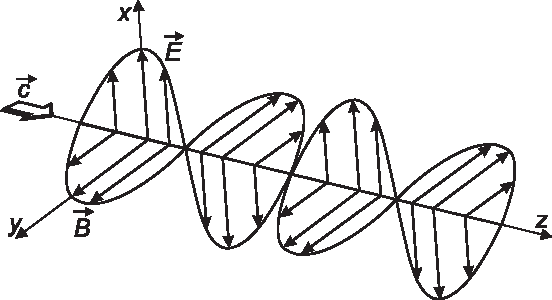
\includegraphics[width=0.58\textwidth]{em_wave.pdf}
    \caption{Fala elektromagnetyczna rozchodząca się w kierunku $z$.
             Źródło:~\cite{skrypt}.}\label{fig:em_wave}
\end{figure}

Wiązkę rozchodzącą się wzdłuż $z$ opisują składowe pola elektrycznego~\cite{skrypt}:
\begin{align}
    E_x &= E_{0x}\cos\!\left(2\pi\!\left(\frac{t}{T} - \frac{z}{\lambda}\right)\right),
    \label{eq:Ex} \\
    E_y &= E_{0y}\cos\!\left(2\pi\!\left(\frac{t}{T} - \frac{z}{\lambda}\right)
           + \varphi\right),
    \label{eq:Ey}
\end{align}
gdzie $E_{0x}$, $E_{0y}$ --- amplitudy składowych, $T$ --- okres drgań,
$\lambda$ --- długość fali, a $\varphi$ --- wzajemne przesunięcie fazowe.
Dla $\varphi = n\pi$ ($n \in \mathbb{Z}$) koniec wektora $\vec{E}$ drga w stałej
płaszczyźnie --- jest to \emph{polaryzacja liniowa}. Gdy $E_{0x} = E_{0y}$
i $\varphi = (2n+1)\pi/2$, koniec $\vec{E}$ zakreśla okrąg (\emph{polaryzacja kołowa}).
W pozostałych przypadkach zakreśla elipsę (\emph{polaryzacja eliptyczna}).
Zwykłe światło termiczne jest \emph{niespolaryzowane} --- kierunki drgań $\vec{E}$
rozkładają się równomiernie (Rysunek~\ref{fig:polarization_types}).

\begin{figure}[H]
    \centering
    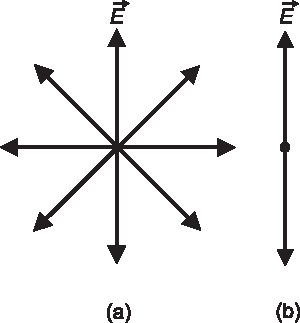
\includegraphics[width=0.42\textwidth]{unpolarized_and_polarized_light.pdf}
    \caption{Przekrój poprzeczny wiązki: (a)~niespolaryzowanej,
             (b)~spolaryzowanej liniowo.
             Źródło:~\cite{skrypt}.}\label{fig:polarization_types}
\end{figure}

\subsection{Prawo Malusa}

Polaryzator liniowy (polaroid) jest materiałem wykazującym \emph{dichroizm} --- pochłania
składową $\vec{E}$ prostopadłą do swojej osi transmisji, przepuszczając jedynie składową
równoległą. Gdy spolaryzowane liniowo światło o natężeniu $I_0$ pada na analizator
ustawiony pod kątem $\theta$ względem płaszczyzny polaryzacji,
natężenie transmitowane opisuje \emph{prawo Malusa}~\cite{skrypt}:
\begin{equation}
    I = I_0\cos^2\!\theta.
    \label{eq:malus}
\end{equation}
Maksimum transmisji ($I = I_0$) odpowiada równoległym osiom obu polaroidów,
wygaszenie ($I = 0$) --- osiom prostopadłym. W praktyce, uwzględniając niezerowe tło
$a_3$ (prąd ciemny detektora, niecałkowita ekstynkcja), mierzony sygnał ma postać:
\begin{equation}
    U(\theta) = a_1\cos^2(\theta + a_2) + a_3,
    \label{eq:malus_fit}
\end{equation}
gdzie $a_1$ --- amplituda, $a_2$ --- przesunięcie kątowe wynikające z odchylenia
osi transmisji polaryzatora od zera skali.

\subsection{Polaryzacja przez odbicie}

Przy odbiciu niespolaryzowanej wiązki od powierzchni dielektrycznej składowa $\vec{E}$
leżąca w płaszczyźnie padania i składowa do niej prostopadła odbijają się z różną
skutecznością --- wiązka odbita jest częściowo spolaryzowana (Rysunek~\ref{fig:brewster}a).
Dla kąta padania równego \emph{kątowi Brewstera} $\theta_B$ promień odbity i załamany
są prostopadłe, a wiązka odbita jest całkowicie spolaryzowana liniowo
(Rysunek~\ref{fig:brewster}b). Z prawa Snella wynika wówczas~\cite{skrypt}:
\begin{equation}
    n = \tan\theta_B,
    \label{eq:brewster}
\end{equation}
gdzie $n$ jest współczynnikiem załamania ośrodka odbijającego.

\begin{figure}[H]
    \centering
    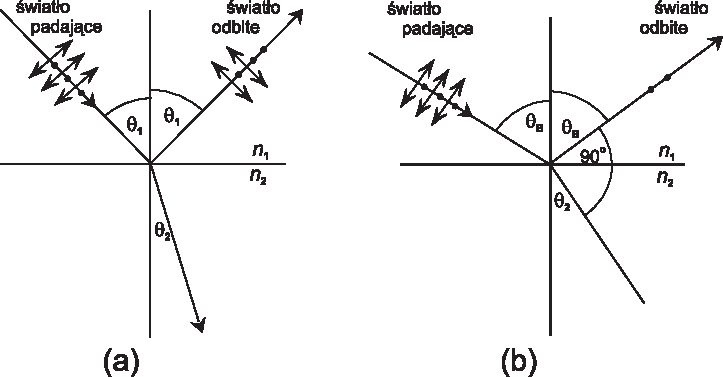
\includegraphics[width=0.65\textwidth]{polarization_by_partial_reflection.pdf}
    \caption{Polaryzacja światła przez odbicie od powierzchni dielektrycznej:
             (a)~częściowa polaryzacja wiązki odbitej i załamanej dla dowolnego kąta
             padania, (b)~całkowita polaryzacja wiązki odbitej dla kąta Brewstera
             $\theta_B$, gdy promień odbity i załamany są prostopadłe.
             Źródło:~\cite{skrypt}.}\label{fig:brewster}
\end{figure}

\subsection{Dwójłomność i płytki fazowe}

Kryształy anizotropowe posiadają dwa różne współczynniki załamania dla promienia
\emph{zwyczajnego} O ($n_O$) i \emph{nadzwyczajnego} E ($n_E$) --- zjawisko
\emph{dwójłomności}. Padająca wiązka ulega rozszczepieniu na dwa ortogonalnie
spolaryzowane promienie poruszające się z różnymi prędkościami
(Rysunek~\ref{fig:birefringent}).

\begin{figure}[H]
    \centering
    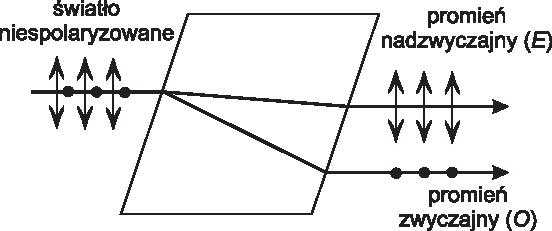
\includegraphics[width=0.60\textwidth]{birefringent_plate.pdf}
    \caption{Bieg promieni w krysztale dwójłomnym: promień zwyczajny O i
             nadzwyczajny E wychodzą z przesunięciem przestrzennym.
             Źródło:~\cite{skrypt}.}\label{fig:birefringent}
\end{figure}

\subsection{Ćwierćfalówka i polaryzacja eliptyczna}

Płytka ćwierćfalowa ($\lambda/4$) jest cienką płytką z kryształu dwójłomnego wyciętą tak,
by jej oś optyczna leżała równolegle do powierzchni. Grubość $d$ jest dobrana tak, aby
różnica faz między promieniami O i E wynosiła~\cite{skrypt}:
\begin{equation}
    \varphi = \frac{2\pi d}{\lambda}\,|n_O - n_E| = \frac{\pi}{2}.
    \label{eq:qwp}
\end{equation}
Na płytce wyróżnia się dwa wzajemnie prostopadłe kierunki drgań zwane \emph{azymutami}.
Jeśli spolaryzowane liniowo światło pada na ćwierćfalówkę pod kątem $\theta$
do jej azymutów, amplitudy składowych wzdłuż osi szybkiej i wolnej wynoszą
odpowiednio $E_{0x} = E_0\cos\theta$ i $E_{0y} = E_0\sin\theta$.
Dla \emph{idealnej} ćwierćfalówki ($\varphi = \pi/2$) składowe te doznają
przesunięcia fazy o $\pi/2$, tworząc elipsę polaryzacji o stosunku półosi
$e = b/a$ danym wzorem~\cite{skrypt}:
\begin{equation}
    e = |\tan\theta|,
    \label{eq:ellipticity}
\end{equation}
gdzie kąt $\theta = 45^{\circ}$ daje polaryzację kołową ($e = 1$), a $\theta = 0^{\circ}$
lub $90^{\circ}$ --- polaryzację liniową ($e = 0$).
Wzór~\eqref{eq:ellipticity} obowiązuje przy założeniu $\varphi = \pi/2$;
dla rzeczywistej płytki, w której $\varphi$ może odbiegać od $\pi/2$ ze względu
na dyspersję materiału lub niedokładność wykonania, eliptyczność jest funkcją
zarówno $\theta$, jak i $\varphi$~\cite{skrypt}.
Azymuty ćwierćfalówki wyznacza się, umieszczając ją między skrzyżowanymi polaryzatorami
i obracając płytkę do uzyskania minimum transmisji --- odpowiada ono ustawieniu,
w~którym azymut płytki pokrywa się z osią transmisji jednego z polaryzatorów.

\subsection{Półfalówka}

Płytka półfalowa ($\lambda/2$) wytwarza między promieniami O i E różnicę faz $\varphi = \pi$,
co obraca płaszczyznę polaryzacji światła liniowego o kąt $2\phi$, gdzie $\phi$ jest
kątem między kierunkiem polaryzacji a azymutami płytki. Ponieważ $\lambda/2 = 2\cdot\lambda/4$,
półfalówkę można złożyć z dwóch ćwierćfalówek ustawionych tak, aby ich azymuty
tworzyły kąt $45^{\circ}$~\cite{skrypt}.

% -------------------------------------------
\section{Opis układu pomiarowego}
% -------------------------------------------

\begin{figure}[H]
    \centering
    
\includegraphics[width=0.82\textwidth]{schema.jpg}
    \caption{Zdjęcie układu doświadczalnego na ławie optycznej.}\label{fig:schema}
\end{figure}

Do przeprowadzenia pomiarów wykorzystano następujące przyrządy:
\begin{itemize}
    \item wysokociśnieniowa lampa rtęciowa z zasilaczem i diafragmą --- źródło
          monochromatycznego światła żółtego ($\lambda = \SI{578}{\nano\meter}$),
    \item filtr interferencyjny dla żółtej linii rtęci,
    \item dwa polaryzatory liniowe (polaroidy) osadzone w uchwytach z podziałką
          kątową, umożliwiającą odczyt kąta z dokładnością $\SI{1}{\degree}$,
    \item dwie płytki ćwierćfalowe $\lambda/4$ osadzone w uchwytach z podziałką
          kątową,
    \item soczewka skupiająca do formowania wiązki,
    \item detektor promieniowania --- element światłoczuły ze wzmacniaczem
          i miernikiem uniwersalnym (woltomierzem).
\end{itemize}
Wszystkie elementy zamontowane są na ławie optycznej, co zapewnia ich
współosiowość. Uchwyty polaryzatorów i płytek ćwierćfalowych umożliwiają
obrót wokół osi wiązki; skale kątowe pozwalają odczytać kąt ustawienia
z niepewnością $u_\theta = \SI{1}{\degree}$.

% -------------------------------------------
\section{Procedura pomiarowa}
% -------------------------------------------

Przed przystąpieniem do pomiarów właściwych usunięto ćwierćfalówki i analizator
z ławy, a następnie ustawiono pozostałe elementy (lampę, filtr, diafragmę,
polaryzator, soczewkę i detektor) tak, aby uzyskać dobre oświetlenie detektora.
Zmierzono wskazanie miernika przy zasłoniętej wiązce (tło, prąd ciemny miernika).

\subsection{Polaryzacja liniowa --- prawo Malusa}

Polaryzator ustawiono w pozycji $0^{\circ}$ i wstawiono analizator. Obracając
analizator od $-90^{\circ}$ do $90^{\circ}$ co $5^{\circ}$, zapisywano wskazanie
woltomierza. W okolicach minimum i maksimum zagęszczono pomiary do co $2^{\circ}$,
aby dokładniej zlokalizować ekstrema.

\subsection{Wyznaczenie azymutów ćwierćfalówki QWP1}

Skrzyżowano polaryzatory (analizator prostopadle do polaryzatora) i wstawiono
między nie pierwszą ćwierćfalówkę. Obracając ćwierćfalówkę w szerokim zakresie
kątów, zlokalizowano przybliżone położenia minimum i maksimum transmisji.
Następnie w otoczeniu każdego ekstremum wykonano pomiary co $1^{\circ}$,
aby wyznaczyć azymuty płytki z możliwie dużą dokładnością.

\subsection{Polaryzacja kołowa}

Usunięto analizator. Ustawiono ćwierćfalówkę QWP1 tak, aby kąt między osią
transmisji polaryzatora a azymutami płytki wynosił $45^{\circ}$, po czym
wstawiono analizator. Obracając analizator od $-90^{\circ}$ do $90^{\circ}$
co $5^{\circ}$, sprawdzono, czy natężenie jest stałe niezależnie od kąta
analizatora, co jest charakterystyczne dla polaryzacji kołowej.

\subsection{Polaryzacje eliptyczne}

Powtórzono procedurę z punktu~3 dla dwóch innych ustawień ćwierćfalówki QWP1.
Płytkę ustawiono w pozycjach $-12^{\circ}$ i $-42^{\circ}$ na skali,
co odpowiada kątowi $\theta_\text{rel} = |\text{ustawienie} - \phi_A| = 15^{\circ}$
względem azymutu po obu jego stronach. Dla każdego ustawienia zmierzono
zależność natężenia od kąta analizatora od $-90^{\circ}$ do $90^{\circ}$
co $5^{\circ}$.

\subsection{Wyznaczenie azymutów ćwierćfalówki QWP2}

Analogicznie do punktu~2, wyznaczono azymuty drugiej ćwierćfalówki QWP2,
zastępując QWP1 przez QWP2 między skrzyżowanymi polaryzatorami.

\subsection{Układ dwóch ćwierćfalówek jako półfalówka}

Wstawiono obie ćwierćfalówki między polaryzatory, ustawiając każdą z nich
w pozycji odpowiadającej jej azymutowi A (ĆF1 przy $-27^{\circ}$, ĆF2 przy $-36^{\circ}$
na skalach), co zgodnie z warunkiem złożenia półfalówki powinno dawać układ
równoważny półfalówce~\cite{skrypt}.
Obracając analizator od $-90^{\circ}$ do $90^{\circ}$ co $5^{\circ}$, sprawdzono,
czy układ przywraca polaryzację liniową, i wyznaczono kierunek polaryzacji
wyjściowej.



% -------------------------------------------
\section{Wyniki pomiarów}
% -------------------------------------------

We wszystkich pomiarach niepewność odczytu kąta wynosi $u_\theta = 1^{\circ}$,
a niepewność wskazania woltomierza $u_I = \SI{0{,}1}{mV}$.
Wskazanie miernika przy zasłoniętej wiązce (tło) wynosiło poniżej progu odczytu.

\subsection{Polaryzacja liniowa}

Zmierzono natężenie światła w funkcji kąta analizatora $\theta$ w zakresie
od $-90^{\circ}$ do $90^{\circ}$, zagęszczając pomiary do co $2^{\circ}$ w okolicach
ekstremów. Wyniki przedstawia Rysunek~\ref{fig:wyniki_lin}.

\begin{figure}[H]
    \centering
    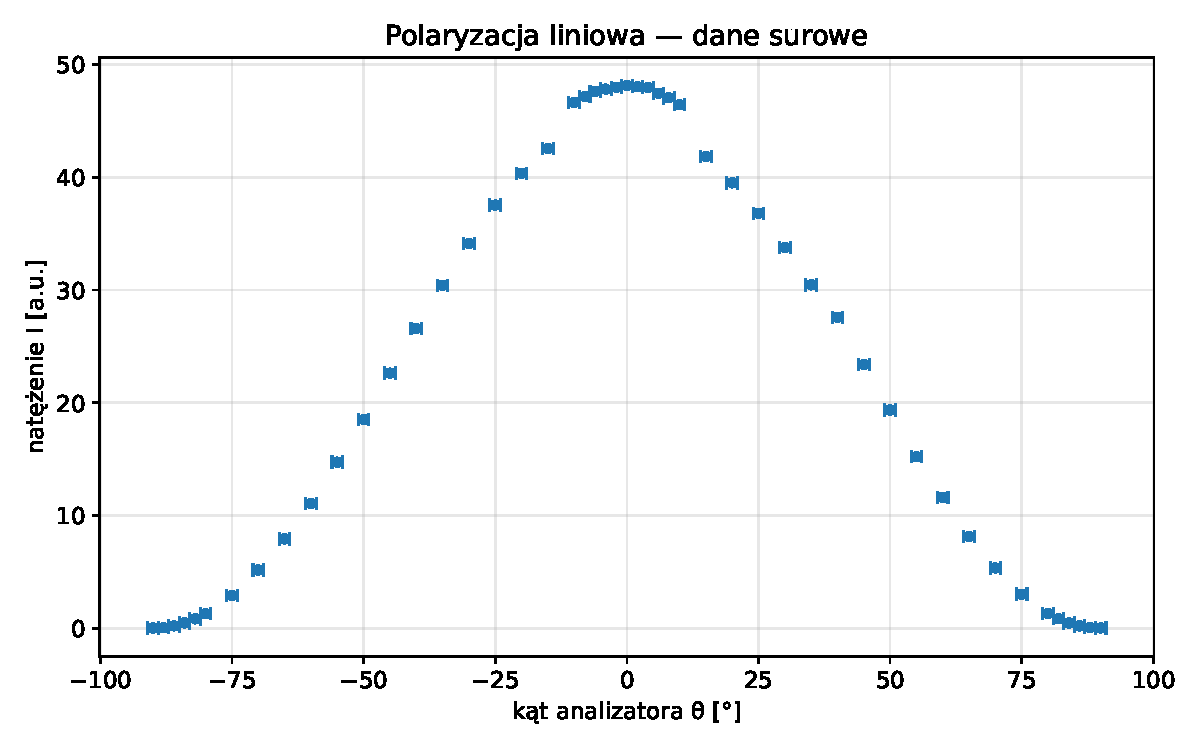
\includegraphics[width=0.82\textwidth]{linear_polarization_raw.pdf}
    \caption{Natężenie światła w funkcji kąta analizatora --- polaryzacja liniowa.
             Słupki błędów odpowiadają niepewnościom $u_\theta = 1^{\circ}$
             i $u_I = \SI{0{,}1}{mV}$.}%
    \label{fig:wyniki_lin}
\end{figure}

\subsection{Azymuty ćwierćfalówki QWP1}

Przy skrzyżowanych polaryzatorach zmierzono natężenie w okolicach minimum
i maksimum transmisji co $1^{\circ}$. Wyniki zestawiono
w Tabeli~\ref{tab:qwp1} i przedstawiono na Rysunku~\ref{fig:wyniki_qwp1}.

\begin{table}[H]
    \centering
    \caption{Pomiary natężenia w otoczeniu ekstremów transmisji dla QWP1
             ($u_\theta = 1^{\circ}$, $u_I = \SI{0{,}1}{mV}$).}\label{tab:qwp1}
    \begin{tabular}{SS@{\quad}SS}
        \toprule
        \multicolumn{2}{c}{Okolice maksimum} & \multicolumn{2}{c}{Okolice minimum} \\
        {$\theta$ [$^{\circ}$]} & {$I$ [mV]} & {$\theta$ [$^{\circ}$]} & {$I$ [mV]} \\
        \midrule
        -30 & 32.41 & 59 &  9.38 \\
        -29 & 32.18 & 60 &  9.44 \\
        -28 & 32.54 & 61 &  9.34 \\
        -27 & 32.54 & 62 &  9.32 \\
        -26 & 32.50 & 63 &  9.32 \\
        -25 & 32.20 & 64 &  9.33 \\
        -24 & 32.25 & 65 &  9.37 \\
        -23 & 32.04 & 66 &  9.42 \\
        \bottomrule
    \end{tabular}
\end{table}

\begin{figure}[H]
    \centering
    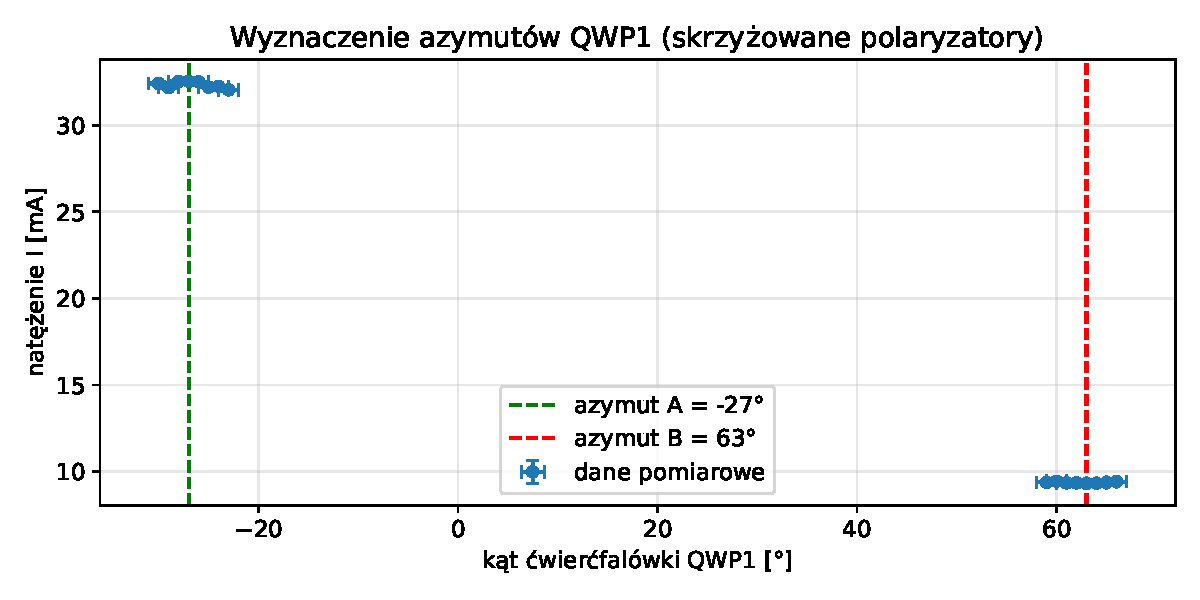
\includegraphics[width=0.82\textwidth]{qwp_schematics.pdf}
    \caption{Natężenie światła w okolicach ekstremów transmisji przy skrzyżowanych
             polaryzatorach --- wyznaczanie azymutów QWP1.}%
    \label{fig:wyniki_qwp1}
\end{figure}

\subsection{Polaryzacja kołowa}

Zmierzono natężenie w funkcji kąta analizatora przy ćwierćfalówce QWP1 ustawionej
pod kątem $45^{\circ}$ do osi transmisji polaryzatora. Wyniki przedstawia
Rysunek~\ref{fig:wyniki_circ}.

\begin{figure}[H]
    \centering
    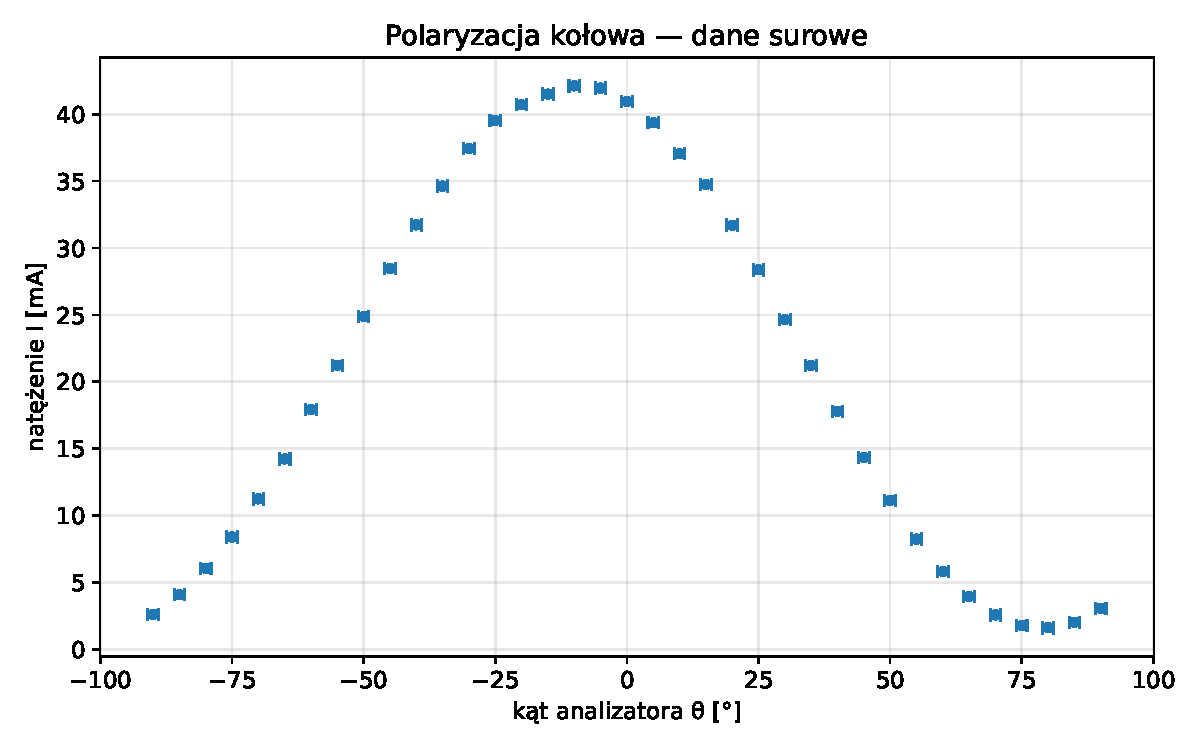
\includegraphics[width=0.82\textwidth]{circular_polarization_raw.pdf}
    \caption{Natężenie światła w funkcji kąta analizatora --- polaryzacja kołowa
             (QWP1 pod kątem $45^{\circ}$ do osi polaryzatora).
             Słupki błędów odpowiadają niepewnościom $u_\theta = 1^{\circ}$
             i $u_I = \SI{0{,}1}{mV}$.}%
    \label{fig:wyniki_circ}
\end{figure}

\subsection{Polaryzacje eliptyczne}

Zmierzono natężenie w funkcji kąta analizatora dla dwóch ustawień ćwierćfalówki
QWP1: przy $-12^{\circ}$ (Rysunek~\ref{fig:wyniki_el1}) oraz $-42^{\circ}$
(Rysunek~\ref{fig:wyniki_el2}) na skali, co odpowiada kątowi względnemu
$\theta_\text{rel} = 15^{\circ}$ między azymutami a osią polaryzatora.

\begin{figure}[H]
    \centering
    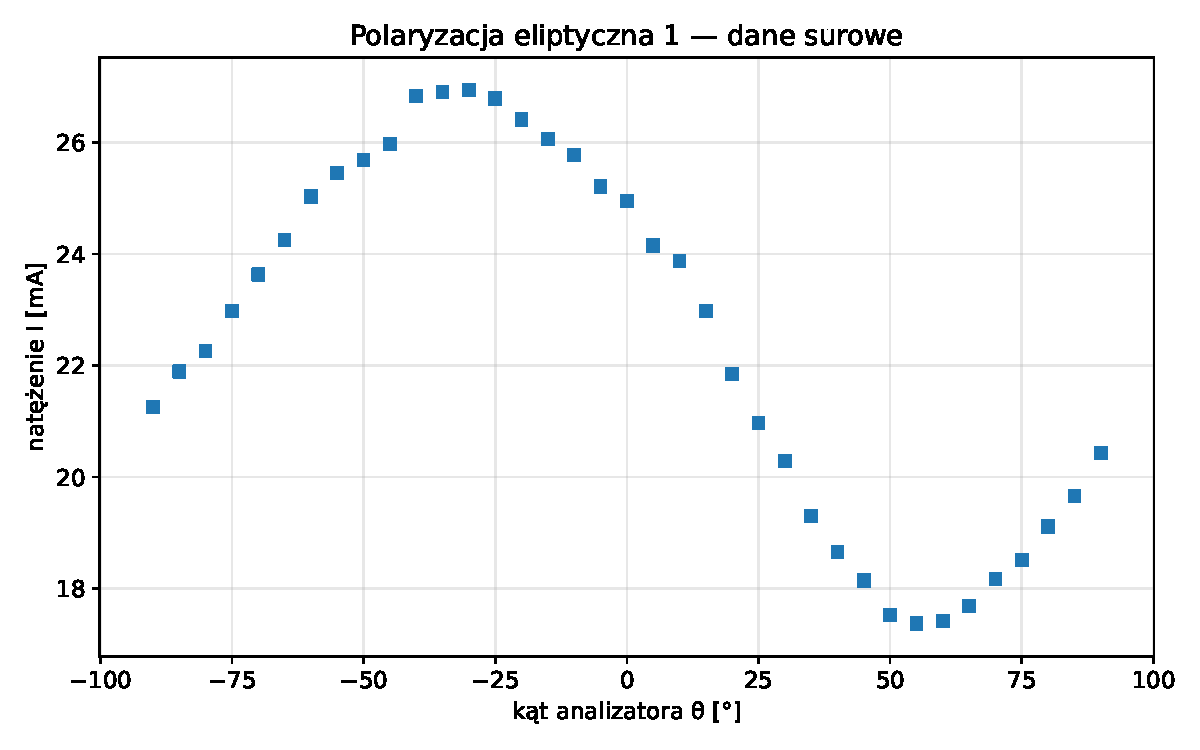
\includegraphics[width=0.82\textwidth]{eliptical_polarization_1_raw.pdf}
    \caption{Natężenie światła w funkcji kąta analizatora --- polaryzacja eliptyczna,
             QWP1 przy $-12^{\circ}$ ($\theta_\text{rel} = 15^{\circ}$ od azymutu).
             Słupki błędów odpowiadają niepewnościom $u_\theta = 1^{\circ}$
             i $u_I = \SI{0{,}1}{mV}$.}%
    \label{fig:wyniki_el1}
\end{figure}

\begin{figure}[H]
    \centering
    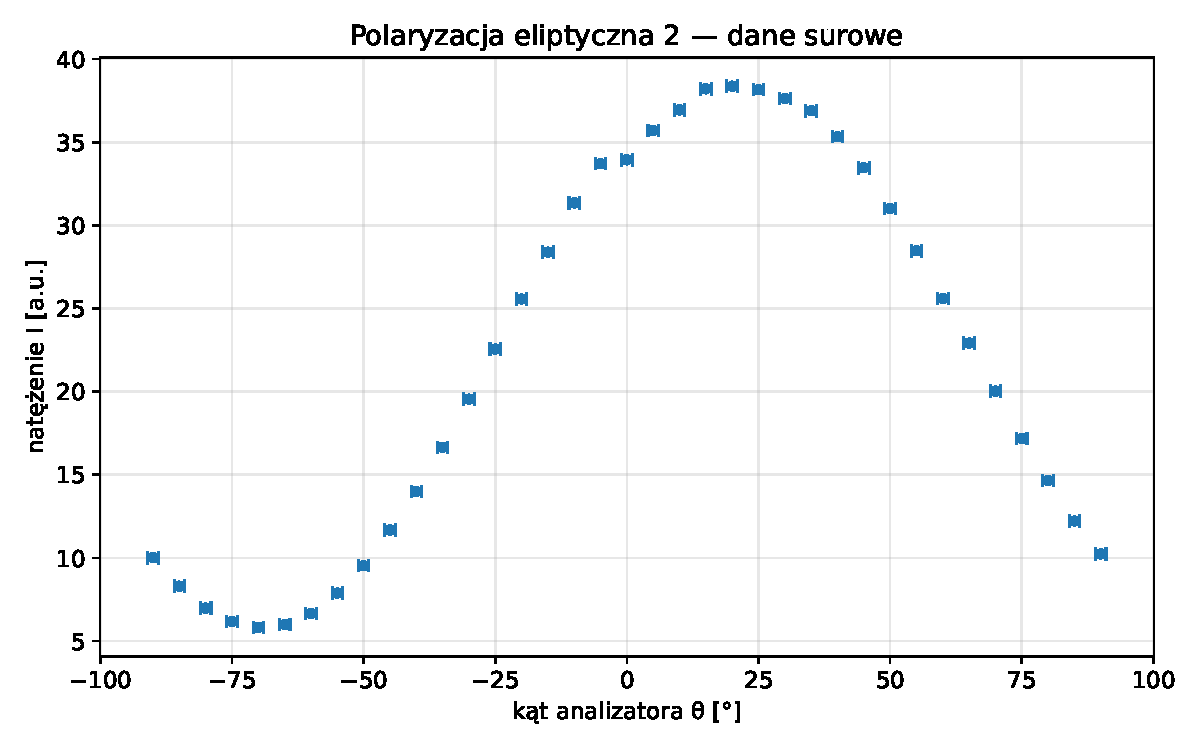
\includegraphics[width=0.82\textwidth]{eliptical_polarization_2_raw.pdf}
    \caption{Natężenie światła w funkcji kąta analizatora --- polaryzacja eliptyczna,
             QWP1 przy $-42^{\circ}$ ($\theta_\text{rel} = 15^{\circ}$ od azymutu, po drugiej stronie).
             Słupki błędów odpowiadają niepewnościom $u_\theta = 1^{\circ}$
             i $u_I = \SI{0{,}1}{mV}$.}%
    \label{fig:wyniki_el2}
\end{figure}

\subsection{Azymuty ćwierćfalówki QWP2}

Analogicznie do pomiarów QWP1 zmierzono natężenie w okolicach ekstremów transmisji
dla drugiej ćwierćfalówki. Wyniki zestawiono w Tabeli~\ref{tab:qwp2}
i przedstawiono na Rysunku~\ref{fig:wyniki_qwp2}.

\begin{table}[H]
    \centering
    \caption{Pomiary natężenia w otoczeniu ekstremów transmisji dla QWP2
             ($u_\theta = 1^{\circ}$, $u_I = \SI{0{,}1}{mV}$).}\label{tab:qwp2}
    \begin{tabular}{SS@{\quad}SS}
        \toprule
        \multicolumn{2}{c}{Okolice maksimum} & \multicolumn{2}{c}{Okolice minimum} \\
        {$\theta$ [$^{\circ}$]} & {$I$ [mV]} & {$\theta$ [$^{\circ}$]} & {$I$ [mV]} \\
        \midrule
        -40 & 30.95 & 51 & 17.66 \\
        -39 & 30.99 & 52 & 17.54 \\
        -38 & 30.91 & 53 & 17.54 \\
        -37 & 32.75 & 54 & 17.53 \\
        -36 & 32.84 & 55 & 17.57 \\
        -35 & 30.91 & 56 & 17.59 \\
        -34 & 31.03 &    &        \\
        \bottomrule
    \end{tabular}
\end{table}

\begin{figure}[H]
    \centering
    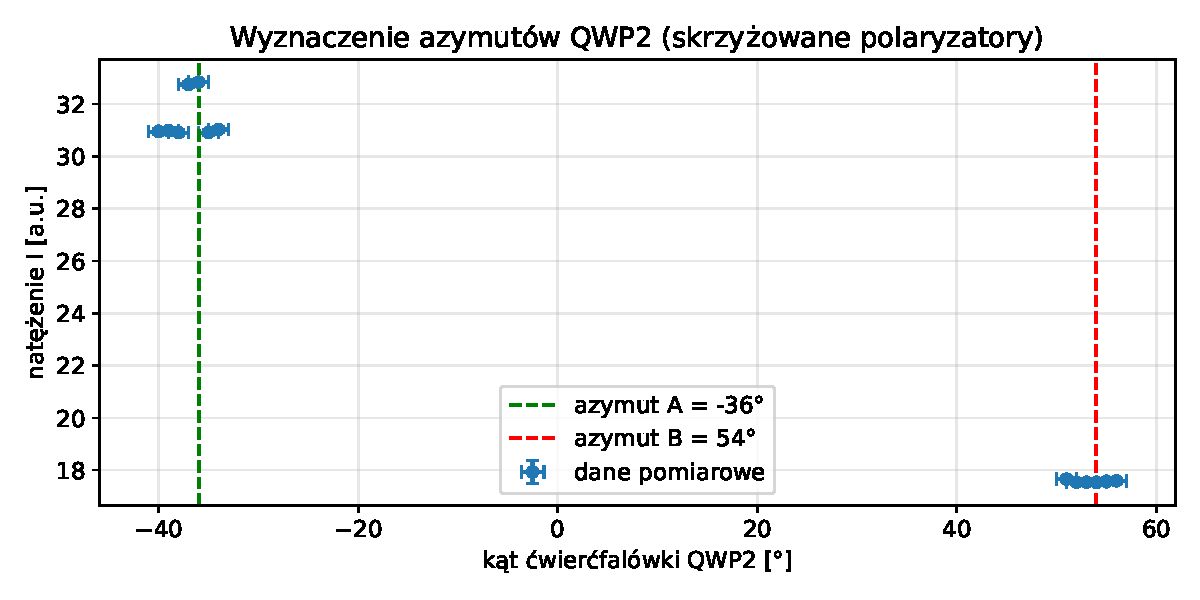
\includegraphics[width=0.82\textwidth]{qwp2_azimuth.pdf}
    \caption{Natężenie światła w okolicach ekstremów transmisji przy skrzyżowanych
             polaryzatorach --- wyznaczanie azymutów QWP2.}%
    \label{fig:wyniki_qwp2}
\end{figure}

\subsection{Układ dwóch ćwierćfalówek jako półfalówka}

Zmierzono natężenie w funkcji kąta analizatora przy obu ćwierćfalówkach ustawionych
tak, aby ich azymuty tworzyły kąt $45^{\circ}$. Wyniki przedstawia
Rysunek~\ref{fig:wyniki_hwp}.

\begin{figure}[H]
    \centering
    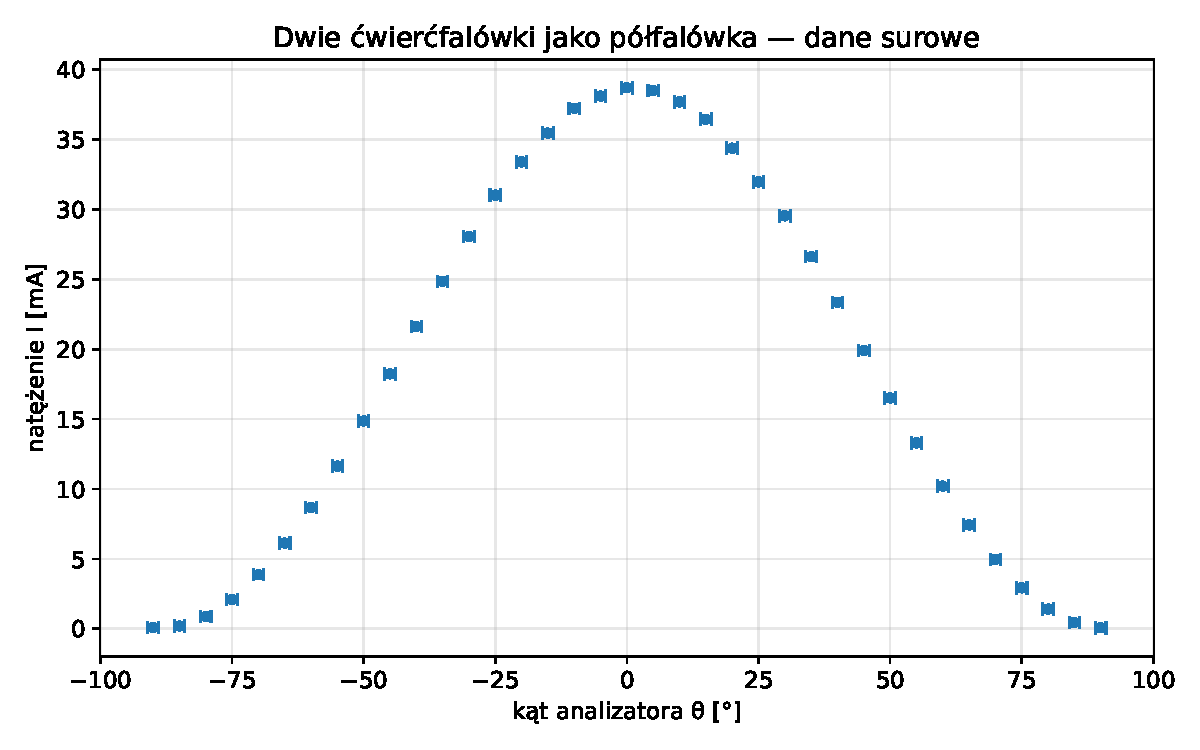
\includegraphics[width=0.82\textwidth]{qwp_both_raw.pdf}
    \caption{Natężenie światła w funkcji kąta analizatora --- układ dwóch
             ćwierćfalówek jako półfalówka.
             Słupki błędów odpowiadają niepewnościom $u_\theta = 1^{\circ}$
             i $u_I = \SI{0{,}1}{mV}$.}%
    \label{fig:wyniki_hwp}
\end{figure}



% -------------------------------------------
\section{Opracowanie wyników}
% -------------------------------------------

\subsection{Prawo Malusa}

Do danych z Rysunku~\ref{fig:wyniki_lin} dopasowano krzywą~\eqref{eq:malus_fit}
funkcją \texttt{scipy.optimize.curve\_fit}; niepewności parametrów przyjęto jako
$u_{a_i} = \sqrt{C_{ii}}$, gdzie $C_{ii}$ jest $i$-tym elementem diagonalnym
macierzy kowariancji dopasowania.
Wyniki zestawiono w Tabeli~\ref{tab:malus_fit},
a dopasowaną krzywą przedstawia Rysunek~\ref{fig:anal_lin}.

\begin{table}[H]
    \centering
    \caption{Parametry dopasowania~\eqref{eq:malus_fit} dla pomiaru prawa Malusa.}%
    \label{tab:malus_fit}
    \begin{tabular}{lS[table-format=2.2]@{\,$\pm$\,}S[table-format=1.2]}
        \toprule
        Parametr & \multicolumn{2}{c}{Wartość $\pm$ $u$} \\
        \midrule
        $a_1$ [mV]        & 48.08 & 0.07 \\
        $a_2$ [\textdegree] &  0.3  & 0.1  \\
        $a_3$ [mV]        &  0.04 & 0.05 \\
        \bottomrule
    \end{tabular}
\end{table}

\begin{figure}[H]
    \centering
    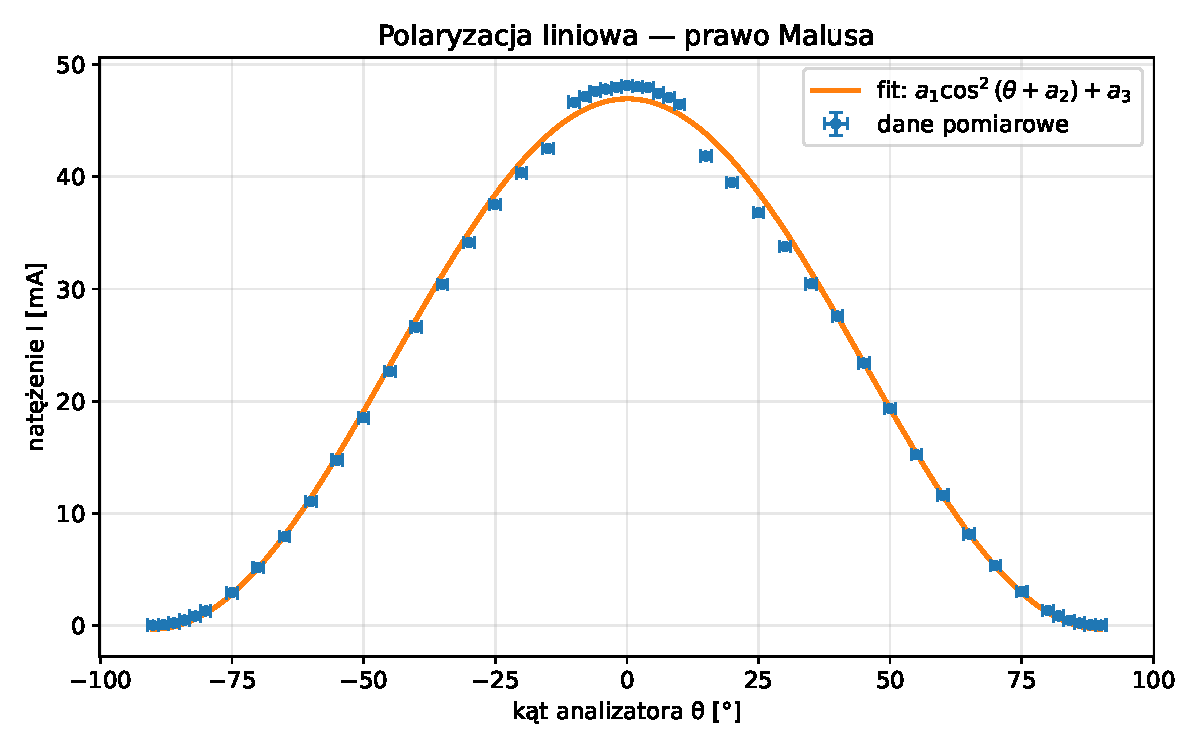
\includegraphics[width=0.72\textwidth]{linear_polarization.pdf}
    \caption{Napięcie fotodetektora w funkcji kąta analizatora dla światła
             za polaryzatorem --- dane pomiarowe z dopasowaną krzywą
             $U(\theta) = a_1\cos^2(\theta + a_2) + a_3$.}%
    \label{fig:anal_lin}
\end{figure}

Tło $a_3 = \SI{0{,}04}{mV}$ jest pomijalnie małe względem amplitudy:
$a_3/(a_1+a_3) \approx 0{,}08\,\%$.
Potwierdza to wysoką jakość polaryzacji liniowej za polaryzatorem.
Kierunek polaryzacji odchyla się od zera skali o $a_2 = {(0{,}3 \pm 0{,}1)}^{\circ}$,
co jest pomijalnie małe.

\subsection{Azymuty ćwierćfalówek}

Azymuty obu płytek ćwierćfalowych wyznaczono z minimów transmisji między
skrzyżowanymi polaryzatorami: przy ustawieniu odpowiadającym azymutowi
ćwierćfalówka nie zmienia stanu polaryzacji, a polaryzacja liniowa jest
całkowicie wygaszana przez analizator.
Wyniki zestawiono w Tabeli~\ref{tab:azymuty}.

\begin{table}[H]
    \centering
    \caption{Azymuty ćwierćfalówek wyznaczone z minimów transmisji między
             skrzyżowanymi polaryzatorami ($u_\phi = 1^{\circ}$).}%
    \label{tab:azymuty}
    \begin{tabular}{lS[table-format=-2.0]S[table-format=2.0]}
        \toprule
        Płytka & {$\phi_A$ [\textdegree]} & {$\phi_B$ [\textdegree]} \\
        \midrule
        ĆF1 & -27 & 63 \\
        ĆF2 & -36 & 54 \\
        \bottomrule
    \end{tabular}
\end{table}

Dla obu płytek $|\phi_B - \phi_A| = 90^{\circ}$, zgodnie z oczekiwaniem ---
azymuty ćwierćfalówki wyznaczają wzajemnie prostopadłe kierunki.
Warto odnotować, że w danych dla QWP2 (Tabela~\ref{tab:qwp2}) wartości przy
$-37^{\circ}$ i $-36^{\circ}$ (odpowiednio $32{,}75$ i $32{,}84$~mV) wyraźnie
odstają od sąsiednich (~$31$~mV), co sugeruje chwilowe wahania miernika w trakcie
pomiaru i stanowi dodatkowe źródło niepewności przy wyznaczaniu $\phi_A$ dla QWP2.

\subsection{Polaryzacja kołowa i eliptyczna}

Eliptyczność doświadczalną obliczono korzystając z faktu, że wartości
$I_\text{min}$ i $I_\text{max}$ intensywności eliptycznie spolaryzowanego
światła mierzonej przez obracany analizator są równe kwadratom długości
półosi elipsy polaryzacji (w jednostkach amplitudy pola):
\begin{equation}
    e_\text{exp} = \frac{b}{a} = \sqrt{\frac{I_\text{min}}{I_\text{max}}}
                 = \sqrt{\frac{a_3}{a_1 + a_3}},
    \label{eq:eexp}
\end{equation}
gdzie $I_\text{min} = a_3$ i $I_\text{max} = a_1 + a_3$ są parametrami
dopasowania~\eqref{eq:malus_fit}. Metodą propagacji niepewności:
\begin{equation}
    u(e_\text{exp}) = \frac{1}{2\,e_\text{exp}\,{(a_1+a_3)}^2}
        \sqrt{a_3^2\,u_{a_1}^2 + a_1^2\,u_{a_3}^2}.
    \label{eq:ueexp}
\end{equation}
Eliptyczność teoretyczną~\eqref{eq:ellipticity} obliczono dla kąta względnego
$\theta_\text{rel} = |\text{ustawienie ĆF} - \phi_A|$
przy założeniu idealnej ćwierćfalówki ($\varphi = \pi/2$):
\begin{equation}
    e_\text{teor} = |\tan\theta_\text{rel}|, \qquad
    u(e_\text{teor}) = \frac{u_{\theta_\text{rel}}}{\cos^2\!\theta_\text{rel}},
    \label{eq:eteor}
\end{equation}
gdzie $u_{\theta_\text{rel}}$ należy wyrazić \emph{w radianach}:
$u_{\theta_\text{rel}} = \sqrt{u_\phi^2 + u_\text{ust}^2}\cdot\tfrac{\pi}{180}
= \sqrt{2}\cdot\tfrac{\pi}{180}\,\text{rad}$
($u_\phi = 1^{\circ}$ --- niepewność wyznaczenia azymutu,
 $u_\text{ust} = 1^{\circ}$ --- niepewność odczytu ustawienia ĆF).

\medskip\noindent\textbf{Polaryzacja kołowa ($\theta_\text{rel} = 45^{\circ}$).}
Wyniki dopasowania dla pomiaru polaryzacji kołowej podano w
Tabeli~\ref{tab:circ_fit}; Rysunek~\ref{fig:anal_circ} przedstawia
dopasowaną krzywą.

\begin{table}[H]
    \centering
    \caption{Parametry dopasowania~\eqref{eq:malus_fit} dla pomiaru polaryzacji kołowej.}%
    \label{tab:circ_fit}
    \begin{tabular}{lS[table-format=2.1]@{\,$\pm$\,}S[table-format=1.1]}
        \toprule
        Parametr & \multicolumn{2}{c}{Wartość $\pm$ $u$} \\
        \midrule
        $a_1$ [mV]          & 40.5 & 0.3 \\
        $a_2$ [\textdegree] & 10.0 & 0.5 \\
        $a_3$ [mV]          &  1.6 & 0.2 \\
        \bottomrule
    \end{tabular}
\end{table}

\begin{figure}[H]
    \centering
    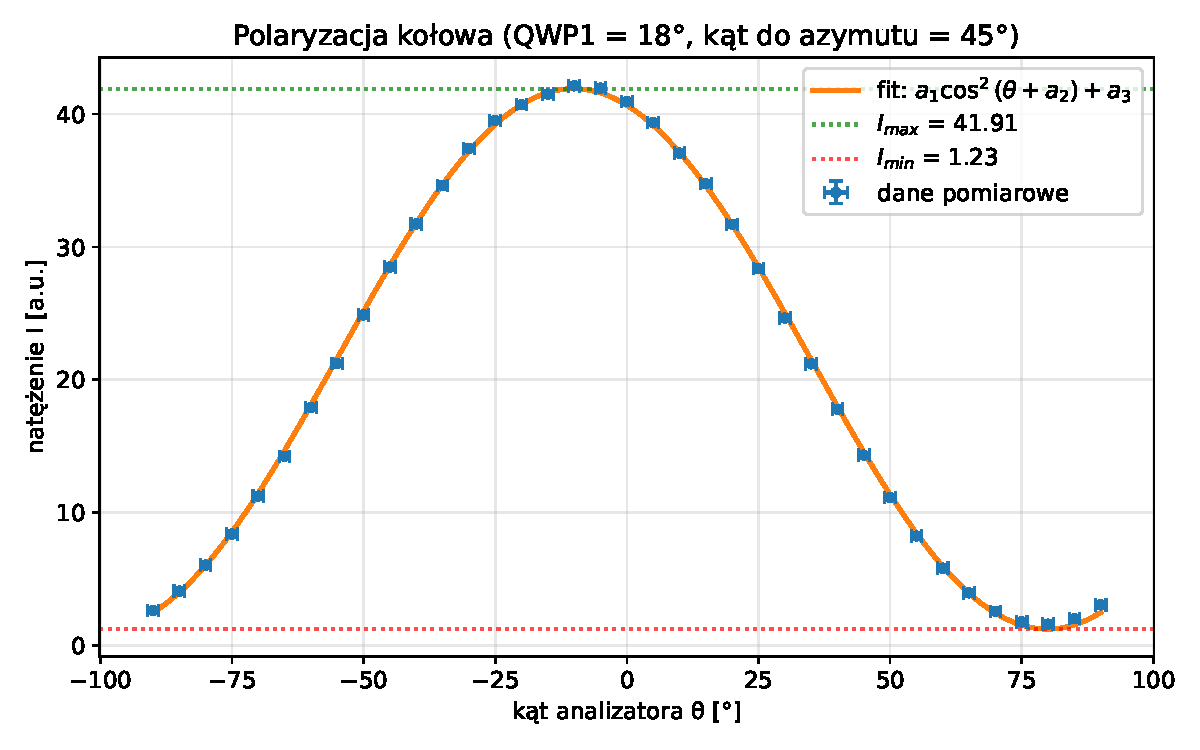
\includegraphics[width=0.72\textwidth]{circular_polarization.pdf}
    \caption{Napięcie fotodetektora w funkcji kąta analizatora dla pomiaru
             polaryzacji kołowej --- dane pomiarowe z dopasowaną krzywą.}%
    \label{fig:anal_circ}
\end{figure}

Ze wzoru~\eqref{eq:eexp}: $I_\text{max} = a_1+a_3 = \SI{42{,}1}{mV}$,
$I_\text{min} = a_3 = \SI{1{,}6}{mV}$, skąd:
\begin{equation}
    e_\text{exp} = \sqrt{\frac{1{,}6}{42{,}1}} = 0{,}195 \pm 0{,}012.
\end{equation}
Eliptyczność teoretyczna dla $\theta_\text{rel} = 45^{\circ}$ ze wzoru~\eqref{eq:eteor}:
\begin{equation}
    e_\text{teor} = |\tan 45^{\circ}| = 1{,}000 \pm 0{,}049.
\end{equation}
Wartości te różnią się istotnie, co wskazuje, że uzyskana polaryzacja jest
daleoka od kołowej. Kierunek głównej osi elipsy wyznaczony z dopasowania:
$\theta_\text{gł} = -a_2 = {(-10 \pm 1)}^{\circ}$.

\medskip\noindent\textbf{Polaryzacje eliptyczne ($\theta_\text{rel} = 15^{\circ}$).}
Dla obu pomiarów ćwierćfalówka ĆF1 odchylona jest o $15^{\circ}$ od azymutu.
Dopasowane krzywe przedstawiają Rysunki~\ref{fig:anal_el1} i~\ref{fig:anal_el2};
parametry dopasowania i wyznaczone eliptyczności zestawiono w
Tabelach~\ref{tab:el_fit} i~\ref{tab:elpol}.

\begin{figure}[H]
    \centering
    \begin{subfigure}[b]{0.48\textwidth}
        \centering
        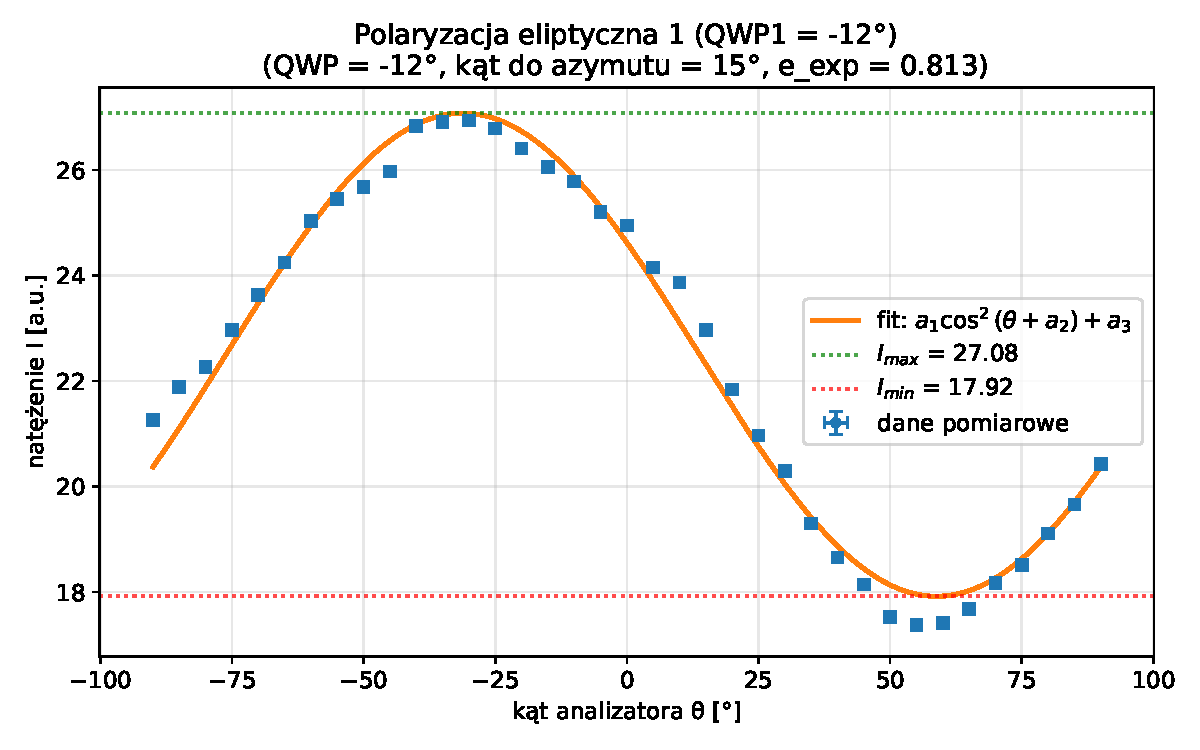
\includegraphics[width=\textwidth]{eliptical_polarization_1.pdf}
        \caption{Pomiar 1 (ĆF1 przy $-12^{\circ}$).}%
        \label{fig:anal_el1}
    \end{subfigure}%
    \hfill
    \begin{subfigure}[b]{0.48\textwidth}
        \centering
        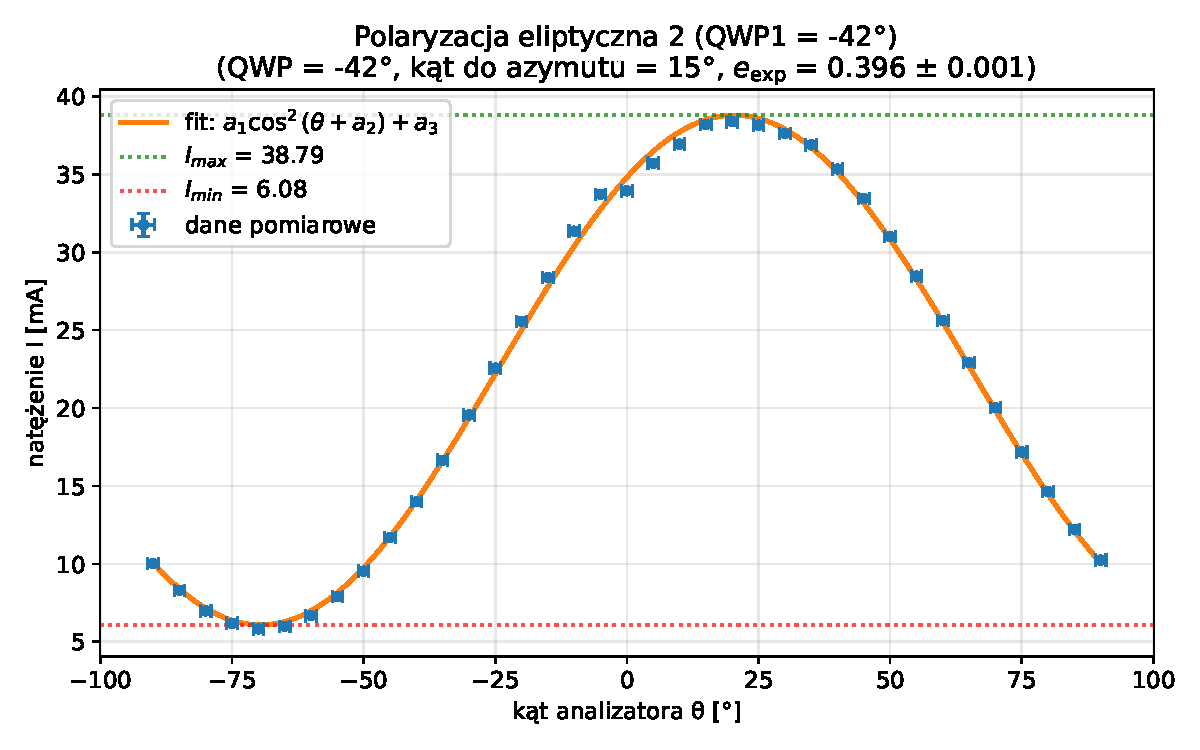
\includegraphics[width=\textwidth]{eliptical_polarization_2.pdf}
        \caption{Pomiar 2 (ĆF1 przy $-42^{\circ}$).}%
        \label{fig:anal_el2}
    \end{subfigure}
    \caption{Napięcie fotodetektora w funkcji kąta analizatora dla obu pomiarów
             polaryzacji eliptycznej ($\theta_\text{rel} = 15^{\circ}$) ---
             dane pomiarowe z dopasowanymi krzywymi.}%
    \label{fig:anal_elpol}
\end{figure}

\begin{table}[H]
    \centering
    \caption{Parametry dopasowania~\eqref{eq:malus_fit} dla pomiarów
             polaryzacji eliptycznej.}%
    \label{tab:el_fit}
    \begin{tabular}{l
                    S[table-format=-2.2]@{\,$\pm$\,}S[table-format=1.2]
                    @{\quad}
                    S[table-format=-2.2]@{\,$\pm$\,}S[table-format=1.2]}
        \toprule
        Parametr & \multicolumn{2}{c}{Pomiar 1} & \multicolumn{2}{c}{Pomiar 2} \\
        \midrule
        $a_1$ [mV]          &  9.16 & 0.05 & 32.71 & 0.05 \\
        $a_2$ [\textdegree] & 31.17 & 0.14 & -20.43 & 0.04 \\
        $a_3$ [mV]          & 17.92 & 0.03 &  6.08 & 0.03 \\
        \bottomrule
    \end{tabular}
\end{table}

\begin{table}[H]
    \centering
    \caption{Porównanie eliptyczności doświadczalnej~\eqref{eq:eexp}
             z teoretyczną~\eqref{eq:eteor} dla pomiarów polaryzacji
             eliptycznej i kołowej.}%
    \label{tab:elpol}
    \begin{tabular}{l
                    S[table-format=1.3]@{\,$\pm$\,}S[table-format=1.3]
                    @{\quad}
                    S[table-format=1.3]@{\,$\pm$\,}S[table-format=1.3]
                    S[table-format=-2.0]}
        \toprule
        Pomiar & \multicolumn{2}{c}{$e_\text{exp}$}
               & \multicolumn{2}{c}{$e_\text{teor}$}
               & {$\theta_\text{gł}$ [\textdegree]} \\
        \midrule
        Kołowa ($45^{\circ}$)       & 0.195 & 0.012 & 1.000 & 0.049 & -10 \\
        Eliptyczna 1 ($15^{\circ}$) & 0.813 & 0.001 & 0.268 & 0.026 & -31 \\
        Eliptyczna 2 ($15^{\circ}$) & 0.396 & 0.001 & 0.268 & 0.026 &  20 \\
        \bottomrule
    \end{tabular}
\end{table}

Kierunek głównej osi elipsy wyznaczono jako $\theta_\text{gł} = -a_2$
(kąt, przy którym natężenie transmitowane przez analizator jest maksymalne).
We wszystkich pomiarach wartości $e_\text{exp}$ odbiegają znacząco
od $e_\text{teor}$, co omówiono w sekcji Wnioski.

\subsection{Układ dwóch ćwierćfalówek jako półfalówka}

Dwie ćwierćfalówki ĆF1 i ĆF2 ustawiono tak, aby tworzyły układ półfalowy.
Wyniki dopasowania zestawiono w Tabeli~\ref{tab:hwp_fit},
a dopasowaną krzywą przedstawia Rysunek~\ref{fig:anal_hwp}.

\begin{table}[H]
    \centering
    \caption{Parametry dopasowania~\eqref{eq:malus_fit} dla pomiaru
             półfalówki złożonej z dwóch ćwierćfalówek.}%
    \label{tab:hwp_fit}
    \begin{tabular}{lS[table-format=2.2]@{\,$\pm$\,}S[table-format=1.2]}
        \toprule
        Parametr & \multicolumn{2}{c}{Wartość $\pm$ $u$} \\
        \midrule
        $a_1$ [mV]          & 38.64 & 0.07 \\
        $a_2$ [\textdegree] &  0.0  & 0.1  \\
        $a_3$ [mV]          &  0.07 & 0.05 \\
        \bottomrule
    \end{tabular}
\end{table}

\begin{figure}[H]
    \centering
    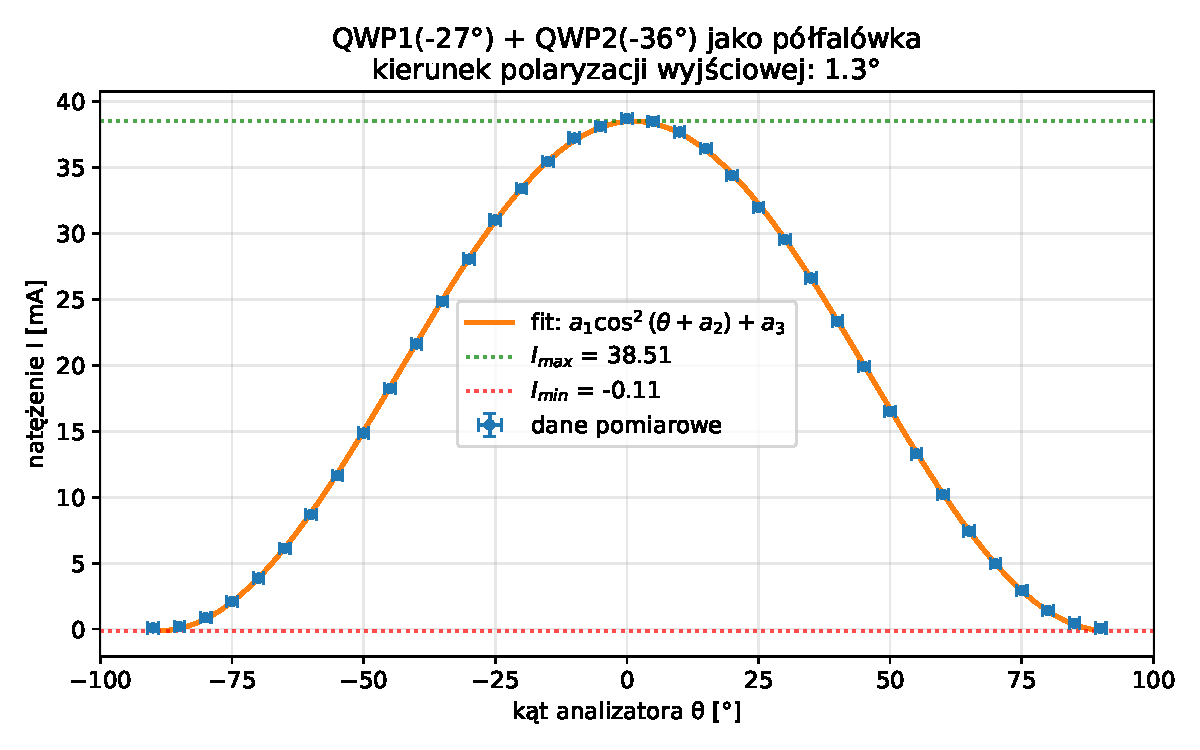
\includegraphics[width=0.72\textwidth]{qwp_both.pdf}
    \caption{Napięcie fotodetektora w funkcji kąta analizatora dla układu
             dwóch ćwierćfalówek jako półfalówki --- dane pomiarowe z
             dopasowaną krzywą.}%
    \label{fig:anal_hwp}
\end{figure}

Wysoki kontrast dopasowania: $a_3/(a_1+a_3) \approx 0{,}18\,\%$,
potwierdza, że wyjściowe światło jest spolaryzowane liniowo.
Kierunek polaryzacji wyjściowej wyznaczony z dopasowania:
\begin{equation}
    \theta_\text{wyj} = -a_2 = {(0{,}0 \pm 0{,}1)}^{\circ}.
\end{equation}
Odczyt ze skali ćwierćfalówki nie jest bezpośrednio kątem osi szybkiej w przestrzeni
fizycznej. Azymut A ($\phi_A$) to odczyt, przy którym oś szybka pokrywa się
z osią transmisji polaryzatora ($0^{\circ}$ fizyczne). Kąt fizyczny osi szybkiej
przy ustawieniu $X$ na skali wynosi zatem:
\begin{equation}
    \varphi_\text{fiz} = X - \phi_A.
    \label{eq:phi_fiz}
\end{equation}
Dla obu ćwierćfalówek ustawionych na ich azymuty:
\begin{align*}
    \varphi_1 &= (-27^{\circ}) - (-27^{\circ}) = 0^{\circ}, \\
    \varphi_2 &= (-36^{\circ}) - (-36^{\circ}) = 0^{\circ}.
\end{align*}
Obie osie szybkie są równoległe i skierowane wzdłuż $0^{\circ}$ fizycznego.
Efektywny azymut złożonej półfalówki wynosi $\phi_\text{eff} = 0^{\circ}$,
a przewidywany kierunek wyjściowy~\cite{skrypt}:
\begin{equation}
    \theta_\text{wyj}^\text{teor} = 2\phi_\text{eff} - \theta_\text{we}
        = 2\cdot 0^{\circ} - 0^{\circ} = 0^{\circ},
    \qquad u(\theta_\text{wyj}^\text{teor}) = 2u_\phi = 2^{\circ}.
\end{equation}
Wynik doświadczalny $\theta_\text{wyj} = (0{,}0 \pm 0{,}1){}^{\circ}$
jest zgodny z przewidywaniem teorii w granicach niepewności.

% -------------------------------------------
\section{Wnioski}
% -------------------------------------------

\subsection{Prawo Malusa}\label{sec:wnioski_malus}

Pomiar transmisji polaryzatora liniowego w funkcji kąta analizatora potwierdził
prawo Malusa~\eqref{eq:malus}. Stosunek tła do maksymalnej intensywności
$a_3/(a_1+a_3) \approx 0{,}08\,\%$ wskazuje, że zastosowany polaryzator wytwarza
polaryzację liniową bardzo wysokiej jakości. Kierunek polaryzacji pokrywa się z zerem
skali analizatora z dokładnością $0{,}3^{\circ}$.
Zauważono, że wskazania woltomierza wykazywały wahania rzędu kilku procent nawet
przy stałym kącie analizatora --- istotnym źródłem błędu jest zatem niestabilność
lamp rtęciowej oraz fluktuacje elektroniczne toru detekcji. Przyjęta niepewność
$u_I = \SI{0{,}1}{mV}$ jest w tych warunkach niedoszacowana; rzeczywista niepewność
pojedynczego pomiaru intensywności może sięgać ponad $10\,\%$ wartości odczytu.
Mimo to dopasowanie prawa cos$^2$ do gęstej siatki punktów uśrednia fluktuacje
i daje wiarygodny wynik.

\subsection{Azymuty ćwierćfalówek}

Wyznaczone azymuty obu płytek spełniają warunek prostopadłości
$|\phi_B - \phi_A| = 90^{\circ}$, zgodnie z teorią.
Potwierdza to poprawność metody wyznaczania azymutów z minimów transmisji między
skrzyżowanymi polaryzatorami. Wahania miernika utrudniały precyzyjne ustalenie
położenia minimum, co przekłada się na niepewność $u_\phi = 1^{\circ}$ i jest
dominującym źródłem błędu w dalszych pomiarach eliptyczności.

\subsection{Polaryzacja kołowa}

Zmierzona eliptyczność $e_\text{exp} = 0{,}195 \pm 0{,}012$ istotnie odbiega od
wartości teoretycznej $e_\text{teor} = 1{,}000$ dla polaryzacji kołowej.
Rozbieżność ta wynika z błędnej interpretacji azymutów wyznaczonych metodą
skrzyżowanych polaryzatorów.

Natężenie przechodzące przez układ złożony z polaryzatora, ćwierćfalówki
i skrzyżowanego analizatora wynosi~\cite{skrypt}:
\begin{equation}
    I(\varphi) = \tfrac{I_0}{2}\sin^2(2\varphi),
    \label{eq:qwp_cross}
\end{equation}
gdzie $\varphi$ jest kątem między osią szybką płytki a osią transmisji polaryzatora.
Wynika stąd, że:
\begin{itemize}
    \item \textbf{maksimum} transmisji odpowiada $\varphi = 45^{\circ}$ ---
          oś szybka pod kątem $45^{\circ}$ do polaryzatora;
    \item \textbf{minimum} transmisji odpowiada $\varphi = 0^{\circ}$ lub $90^{\circ}$ ---
          oś szybka równoległa lub prostopadła do polaryzatora.
\end{itemize}
Azymut~A (odczyt $-27^{\circ}$) jest zatem pozycją \emph{maksimum}, czyli
odpowiada $\varphi = 45^{\circ}$ --- osi szybkiej już pod kątem $45^{\circ}$
do polaryzatora. Ponieważ właśnie $\varphi = 45^{\circ}$ jest warunkiem koniecznym
do wytworzenia polaryzacji kołowej, prawidłowym ustawieniem ćwierćfalówki był
odczyt azymutu~A ($-27^{\circ}$), a nie $-27^{\circ} + 45^{\circ} = 18^{\circ}$.

Ustawiając ćwierćfalówkę na $18^{\circ}$, obrócono jej oś szybką do pozycji
$\varphi = 90^{\circ}$ względem polaryzatora. W tej konfiguracji wejściowa
fala liniowo spolaryzowana biegnie wyłącznie wzdłuż jednej osi głównej płytki
i nie ulega rozkładowi na dwie ortogonalne składowe --- ćwierćfalówka nie zmienia
stanu polaryzacji. Wyjściowe światło pozostaje liniowo spolaryzowane, co wyjaśnia
uzyskane $e_\text{exp} \approx 0{,}17 \approx 0$ zamiast oczekiwanego $e = 1$.

\subsection{Polaryzacje eliptyczne}

Dla obu pomiarów z $\theta_\text{rel} = 15^{\circ}$ teoria przewiduje
$e_\text{teor} = 0{,}268 \pm 0{,}026$, natomiast doświadczalnie uzyskano
$e_\text{exp} = 0{,}813 \pm 0{,}001$ (pomiar~1) i $e_\text{exp} = 0{,}396 \pm 0{,}001$
(pomiar~2). Obie wartości znacząco odbiegają od teorii, a niesymetria między nimi
--- dwa ustawienia o tym samym $|\theta_\text{rel}|$ dają różne $e_\text{exp}$ ---
wskazuje na efekty systematyczne wykraczające poza prosty błąd kąta.
Do rozbieżności przyczyniają się wahania intensywności źródła powyżej $10\,\%$
wartości odczytu: w pomiarze~1, gdzie $a_1 \approx \SI{9{,}6}{mV}$ (płytka sygnału
względem tła), fluktuacje rzędu kilku dziesiętnych $\text{mV}$ stanowią znaczny
ułamek amplitudy i mogą istotnie zawyżyć $e_\text{exp}$ lub je zaniżyć.
Dodatkową przyczyną jest najprawdopodobniej nieidealne opóźnienie fazowe ćwierćfalówki
(jak w pomiarze polaryzacji kołowej) lub niejednorodność kryształu wzdłuż kierunków
odpowiadających dwóm symetrycznym ustawieniom.
Należy też odnotować, że niepewności $\pm 0{,}001$ przy $e_\text{exp}$ są formalne
--- wynikają wprost z macierzy kowariancji dopasowania przy założeniu $u_I = \SI{0{,}1}{mV}$
--- i są zaniżone z tego samego powodu, co niepewności pozostałych parametrów
(zob.~sekcję~\ref{sec:wnioski_malus}).
Jakościowo efekt działania ćwierćfalówki został jednak potwierdzony: przy każdym
ustawieniu natężenie za analizatorem wykazuje zależność $\cos^2$ z niezerowym
minimum, świadcząc o polaryzacji eliptycznej.

\subsection{Układ dwóch ćwierćfalówek jako półfalówka}

Układ dwóch ćwierćfalówek przepuścił światło o polaryzacji liniowej
z kontrastem $a_3/(a_1+a_3) \approx 0{,}18\,\%$.
Wyznaczony kierunek polaryzacji wyjściowej $\theta_\text{wyj} = (0{,}0 \pm 0{,}1){}^{\circ}$
jest zgodny z przewidywaniem teorii
$(0{,}0 \pm 2{,}0){}^{\circ}$
wyznaczonym przy użyciu fizycznych kątów osi szybkich~\eqref{eq:phi_fiz}:
obie ćwierćfalówki były ustawione na swoje azymuty A, co oznacza,
że ich osie szybkie pokrywały się z osią transmisji polaryzatora ($0^{\circ}$ fizyczne).
Złożony układ dwóch równoległych ćwierćfalówek jest równoważny półfalówce
w $0^{\circ}$, która nie obraca polaryzacji wejściowej zgodnej z tą osią.
Warto zauważyć, że układ dwóch ćwierćfalówek o \emph{dowolnym} wzajemnym ustawieniu
zawsze zachowuje polaryzację liniową --- zmienia jedynie jej kierunek (wynika to
z algebry macierzy Jonesa); dlatego wysoki kontrast wyjściowy jest fizycznie
oczekiwanym wynikiem dla każdej konfiguracji, nie tylko dla warunków półfalówki.
Aby zaobserwować obrót polaryzacji, należałoby ustawić ćwierćfalówki tak, aby ich
fizyczny kąt osi szybkiej różnił się od $0^{\circ}$ (np. ĆF1 przy $0^{\circ}$,
ĆF2 przy $45^{\circ}$ fizycznie), co wymaga odchylenia od azymutów A.

\begin{thebibliography}{9}
\bibitem{skrypt}
    \textit{Skrypt do I Pracowni Fizycznej}, ćwiczenie O8:
    Badanie stanu polaryzacji światła
\end{thebibliography}


\end{document}
